\begin{figure}[!ht]
     \centering
     \def\w{0.3\linewidth}

     \begin{subfigure}{\w}
         \centering
         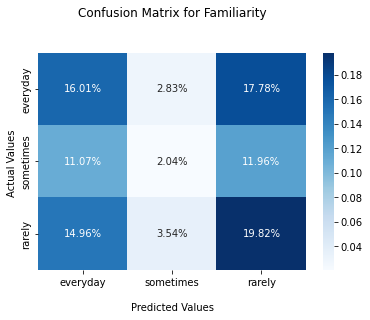
\includegraphics[width=\textwidth]{figures/familiarity_cm.png}
         \caption{\rev{Familiarity}}
         \label{fig:cm_familiarity}
     \end{subfigure}
     \hfill
     \begin{subfigure}{\w}
         \centering
         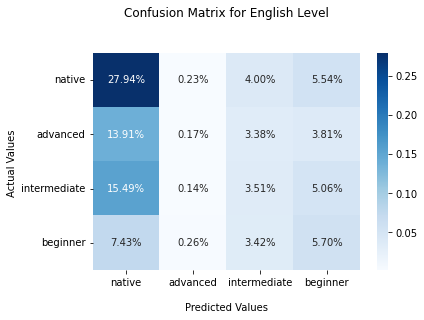
\includegraphics[width=\textwidth]{figures/english_level_cm.png}
         \caption{\rev{English level}}
         \label{fig:cm_engl}
     \end{subfigure}
     \hfill
     \begin{subfigure}{\w}
         \centering
         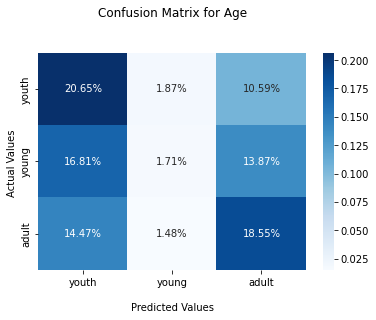
\includegraphics[width=\textwidth]{figures/age_cm.png}
         \caption{\rev{Age}}
         \label{fig:cm_age}
     \end{subfigure}
     \hfill
     \begin{subfigure}{\w}
         \centering
         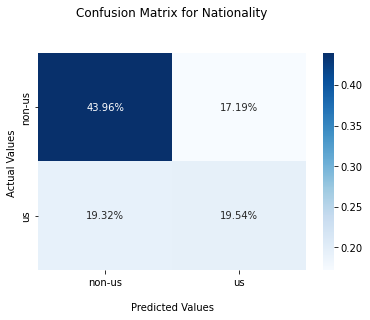
\includegraphics[width=\textwidth]{figures/nationality_cm.png}
         \caption{\rev{Nationality}}
         \label{fig:cm_nat}
     \end{subfigure}
     \hfill
     \begin{subfigure}{\w}
         \centering
         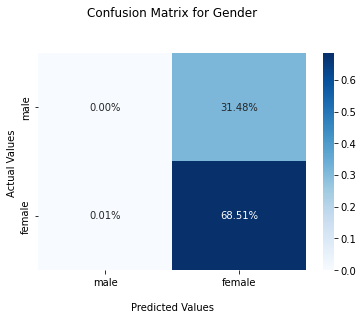
\includegraphics[width=\textwidth]{figures/gender_cm.png}
         \caption{\rev{Gender}}
         \label{fig:cm_gender}
     \end{subfigure}
     \hfill
     \begin{subfigure}{\w}
         \centering
         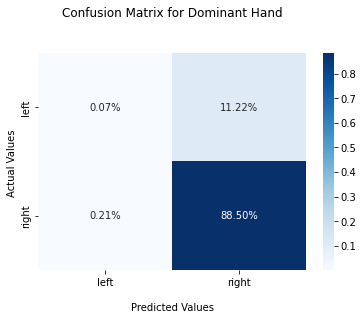
\includegraphics[width=\textwidth]{figures/dominant_hand_cm.png}
         \caption{\rev{Dominant hand}}
         \label{fig:cm_dom}
     \end{subfigure}
     \hfill
     \begin{subfigure}{\w}
         \centering
         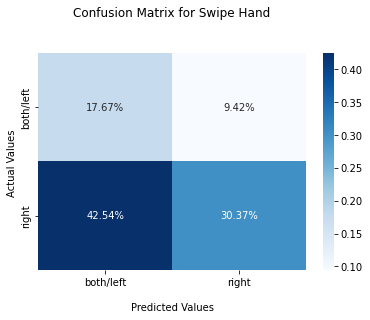
\includegraphics[width=\textwidth]{figures/swipe_hand_cm.png}
         \caption{\rev{Swiping hand}}
         \label{fig:cm_hand}
     \end{subfigure}
     \hfill
     \begin{subfigure}{\w}
         \centering
         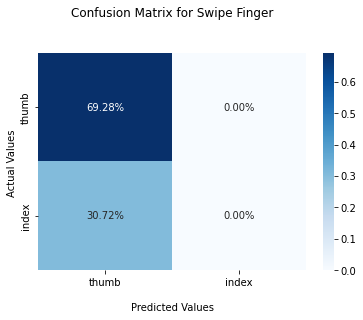
\includegraphics[width=\textwidth]{figures/swipe_finger_cm.png}
         \caption{\rev{Swiping finger}}
         \label{fig:cm_fingder}
     \end{subfigure}
     \hfill
     %% This is to force left-alignment of the last subplot.
     \phantom{
         \begin{subfigure}{\w}
             \centering
             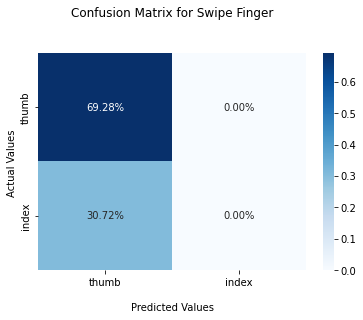
\includegraphics[width=\textwidth]{figures/swipe_finger_cm.png}
             \caption{\rev{Swiping finger}}
             \label{fig:cm_fingder}
         \end{subfigure}
     }

    \caption{\rev{Confusion matrices for the best performing models reported in \protect\autoref{tab:Results}.}}
    \label{fig:confusion_matrices}
\end{figure}
